\section{Задание №8}

Применить метод Монте--Карло к решению первой краевой задачи для двумерного уравнения Лапласа в единичном круге:
$$
        \left\{
\begin{array}{lcr}
        \Delta u=0, \, (x,y)\in D,
\\
        u|_{\delta D}=f(x,y),
\\
        u\in C^2(D), \, f \in C(\delta D),
\\
        D = \{\, x,y \,:\, x^2+y^2 \leqslant 1 \,\}.
\end{array}
        \right.
$$

Для функции $f(x,y)=x^2-y^2$ найти аналитическое решение и сравнить с полученным по методу Монте--Карло.

\subsection{Алгоритм решения задачи}

Построим разностную схему для данной задачи Дирихле. Для этого выберем достаточно мелкую квадратную сетку с шагом~$h$. Координаты узлов пусть будут $x_i = ih$, $y_j = jh$, а значения $u(x_i, y_j)$ и $f(x_i,y_j)$ для краткости обозначим за $u_{i,j}$ и $f_{i,j}$.

\begin{definition}
        Будем называть узел сетки~$(i, j)$ \textit{внутренним}, если он и все четыре соседних с ним узла: $(i-1, j), \ (i + 1, j), \ (i, j - 1), \ (i, j + 1)$ принадлежат области~$D + \delta D$; в противном случае узел $(i, j)$, принадлежащий $D + \delta D$, будем называть \textit{граничным}.
\end{definition}

\begin{figure}[h]
        \noindent
        \centering
        {
                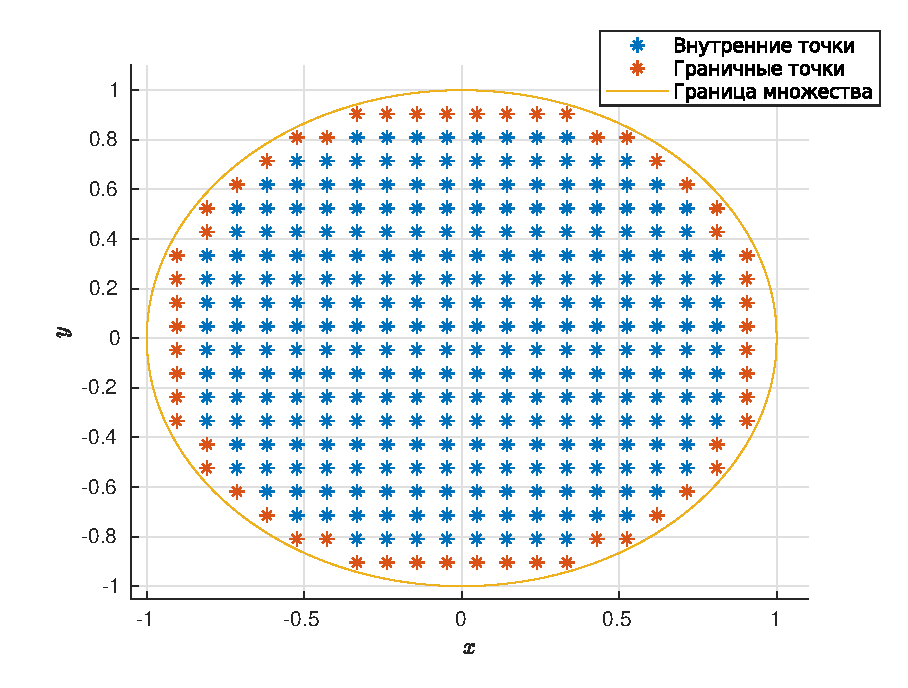
\includegraphics[width=120mm]{task_08/circle.eps}
        }
        \caption{Внешний вид функции $f(x)$}
\end{figure}